
\documentclass[12pt]{article} 
\usepackage[utf8]{inputenc}
\usepackage[slovak]{babel}
\usepackage[hidelinks,unicode = true]{hyperref}
\usepackage{outline}
\usepackage{graphicx}
%\usepackage{biblatex}
%\addbibresource{literatura.bib}
\usepackage{cite}
\usepackage{caption}
\usepackage{listings}
\usepackage{xcolor}
%\usepackage{float} %upevneni tabulky
%\restylefloat{table}
\setcounter{secnumdepth}{3}
\setcounter{tocdepth}{3}
\usepackage{hyperref}
\hypersetup{
    colorlinks=true,
    linkcolor=blue,
    filecolor=magenta,      
    urlcolor=cyan,
}

%===========================================================================
\begin{document}           % Konec preambule a zároveň začátek vlastního textu
\begin{titlepage}
\centering
\Large \textbf{České vysoké učení technické v Praze }\\ Fakulta stavební
\vspace{2cm}

\begin{figure}[h!] %logoCVUT
\centering

\includegraphics[width=7cm]{./img/cvut.png}
\end{figure}
 
\Large \textbf{155UZPR Úvod do zpracování prostorových dat}
\vspace{1cm}

\LARGE  \textbf{ Nasazení vektorových dlaždic při tvorbě katastrální mapy}
\vspace{3cm}

\Large Bc. Linda Kladivová, Bc. Jana Špererová, Bc. Lukáš Kettner, Bc. Martin Hulín \\ \today

 \thispagestyle{empty} %neočísluje první stránku
\end{titlepage}

\tableofcontents    % vytváří  Obsah 
\newpage %začne na nové stránce
%------------------------------------------------------------------------
\section{Úvod}



%------------------------------------------------------------------------
\clearpage 
\section{Popis a rozbor problému}

\subsection{Vektorvý a rastrový formát}
Každý z formátov publikácie priestorových dát má svoje výhody a nevýhody. Je potreba dobre zvážiť umýsel, možnosti a výsledný cieľ publikácie. Rastrové dlaždice majú v porovnaní s vektorovými jednoduchšiu dátovú štruktúru a spracovanie rastrových dát je vo väčšine prípadov jednoduchšie. Veľkou nevýhodou dát v rastrovom formáte sú obmedzené možnosti práce s datami, kedy pri porovnaní s vektorovými dátami pracujeme s obrazom javu a nie konkrétnymi geoprvkami. Ďalšou nevýhodou rastrových dlaždíc je ich veľkosť. Vzhľadom na využitie práce, riešenie má byť aplikované pre dáta celého územia Českej republiky, je práve veľkosť kľúčovým faktorom, ktorý hovorí v prospech vektorových dlaždíc. Z hladiska úložiska vektorové dlaždice zaberajú kapacitne niekoľkonásobne menší (väčšinou) priestor úložiska. Z tohto faktu plynie ďalšia výhoda pri použiti vektorových dlaždíc, úspora datového toku na klientovi, vykreslujú sa dlaždice, ktoré sú v aktuálnom pohľade mapy. 
\newline Ďalším podstatným plusom oproti rastrovým dlaždiciam je možnosť vektorového formátu niesť topologickú informáciu, ktorú môže užívateľ využiť pri následnej práci s dátami a vykonávaní rozličných analýz. Jedným z príkladov je možnosť vykonávať úpravy priamo na strane klienta,  bez nutnosti interakcie so serverom. Táto možnosť je užitočná pri projektoch v oblasti open source mapovania a práci s využitím mapovej služby priamo v teréne. 
\newline K výhodám vektorových dlaždíc patrí aj kartografická generalizácia. V závislosti na úrovni priblíženia (merítku) je možné nastaviť optimalizáciu zobrazenia vektorových dlaždíc. Jednotlivé geoprvky je možné zlúčiť, zjednodušiť či agregovať, tak aby podrobnosť geometrie a atribútového obsahu dlaždíc odpoveda úrovni priblíženia.
\newline Jednou z ďalších výhod vektorových dátach je možná individuálna štylizácia dát na strane klienta, presne podľa jeho požiadavkov, bez toho aby dáta na serveri museli byť zmené.
\newline V prípade modelového príkladu z praxe. Pokiaľ by sme chceli na mobilnom zariadení, v lokalite so slabším internetovým pripojením vykonať jednoduchú analýzu nad mapou vytvorenou z rastrových dlaždíc, sme takmer bez šance na úspech. V prípade použitia vektorových dlaždíc bude možné túto analýzu vykonať.

\subsection{Súčasný stav mapového serveru Marushka}

V súčasnom stave mapový server Marushka slúži k uloženiu, poskytovaniu a aktualizácii mapových dát na území Českej republiky. Všetky dáta publikované touto aplikáciou sú uložené v databázy Informačného systému katastru nemovitostí (ISKN) a v databázy Informačného systému územnej identifikácie (ISÚI). V rámci týchto dvoch databází prebiehajú všetky aktualizácie zobrazených prvkov. Na tieto databáze je následne napojená Publikačná databáza a v nej prebiehajú úpravy geometrií v pravidelných dvojhodinových cykloch. Úpravy sa týkajú zväčša transformácie geometrie , aby bolo možné jej optimálnejšie zobrazovanie a publikácia. Celá logika postupu je na základe databázovej úrovne a je realizovaná pomocou PL/SQL skriptov. Takto upravené dáta sú automaticky exportovaná do WKB súborov. Z týchto preddefinovaných súborov prebieha samotná publikácia dát vo forme rastrových dlaždíc. K aktualizácii katastrálnej mapy dôjde v celom katastrálnom území, pokial sa v ňom objaví zmena.

\begin{center}
   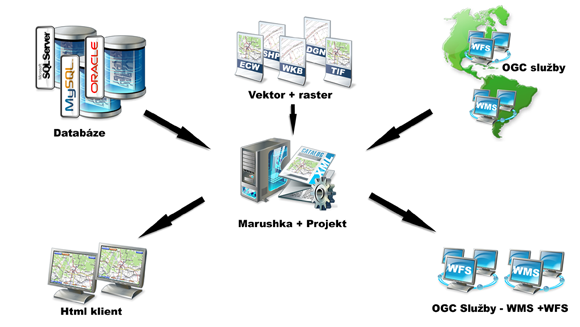
\includegraphics[width=12cm]{./img/Marushka1.png}
   \captionof{figure}{Mapový server Marushka}
\end{center}

 Pre lepšie porozumenie je potrebné objasniť, čo je to WKB súbor. Mapový server Marushka nativne pracuje s týmto vektorovým formátom, Well known Binary (WKB, štandard konsorcia OGC). Tento formát je používaný aj pre implementáciu databázového priestorového úložiska, ktoré je kompatibilné s produktami fy GEOVAP(Geostore), prípadne pre export akéhokoľvek skladu do tzv. file cash. 
 \newline Nad súbormi WKB je možné vybudovať viacúrovňový priestorový index reprezentovaný štruktúrou R-Tree. Tento index výrazne zefektívni priestorový prístup k jednotlivým geometrickým elemoentom. Podrobnejšie informácie je možné nájsť na oficiálne stránke  \href{http://geovap.q2.cz/marushka/cz/produkty-a-sluzby/categoryId/3/souborove-vektorove-formaty-/popis/architektura/2#item15}{ serveru Marushka}.
 \newline Využitie vektorových dlaždíc na mapovom serveri Marushka by viedlo k zjednodušeniu aktualizácie katastrálnej mapy. Aktualizovala by sa len základná dlaždica, v ktorej sa prvok nachádza. To by vylúčilo nutnosť aktualizovať celé katastrálne územie, tým by sa výrazne znížila časová náročnosť pre aktualizáciu dát a aktualne dáta na mapovom serveri Marushka by mali užívatelia k dispozícii takmer ihneď po úprave.

\subsection{Možnosti generování vektorových dlaždic}

 V dnešnej dobe je možnosť tvorby vektorových dlaždíc pomocou niekoľkých nástrojov. 
\newline Spoločnosť Mapbox vytvorila otvorenú špecifikáciu apbox Vector Tile - MVT. Jedná sa o nástroj, ktorý umožňuje tvorbu mapových štýlov pre vektorové dlaždice nad vlastnými dátami. Základná varianta poskytovania mapových dlaždíc je dostupná zdarma. Spoločnosť Mapbox ponúka aj ďalšie nástroje, ktoré môže užívateľ využíť pri tvorbe mapovej aplikácie využívajucej ako podklad vektorové mapové dlaždice. Formát MVT je vyvynutý tak, aby požadované údaje boli súvislo v pamäti a aby vrstvy mahli byť bez úpravy údajov pripojené k dlaždici. Každá dlaždica by mala obsahovať aspoň jednu vrstvu, vrstva aspoň jeden prvok a prvok musí obsahovať pole geometrie. Prvky dlaždíc obsahujú ID, atribúty a geometriu. Geometria môže byť definovaná ako bod, línia či polygón. Geometria sa ukladá vo formáte MVT ako pole čísel x a y. Žačiatok jednej dlaždice je  v ľavom hornom rohu a koniec na dolnom okraji alebo v dolnom pravom rohu ( Mapbox 2017 ).
\newline Ďalšou možnosťou je využitie projektu OpenMap Tiles. Jedná sa o sadu nástrojom pre tvorbu a štylizáciu vektorovej mapy. Tento projekt je nástupcom OSM2VectorTiles projektu. Zahŕňa nástroje pre tvorbu vektorových dlaždíc z OSM ( MVT), nástroj pre správu schémy vektorových dlaždíc ( popis jednotlivých tématických datových vrstiev a atribútov ), nástroj pre predpripravené štýly pre dlaždicové dáta a ich jednoduché prispôsobenie. Tento nástroj je možné využiť na počítači s Windows, MAC či Linux operačným systémom, čož je jeho obrovská výhoda napríklad proti nástroju Tippecanoe, ktorý je dostupný len pre Linux.  
\newline Často používaným spôsobom je už spomenutý nástroj Tippecanoe. Nástroj prevádza jednotlivé dáta z formátu GeoJSON, Geobuf alebo CSV do vektorových mapových dlaždíc. Výstupom je formát so špecifikáciou MBTiles. Je ho možné považovať za SQL databázu, ktorá umožní uloženie vektorových mapových dlaždíc v jednom súbore. Tento nástroj bol využitý pri zobrazení vektorových dlaždíc v rámci nášho projektu. Veľkou výhodou bola dostupnosť podrobnej dokumentácie a vzorových príkladov na  \href{https://github.com/mapbox/tippecanoe}{ GitHub}.

 Pri požiadavku generovania vektorových dlaždíc priamo z databáze Oracle je možné využiť niekoľko postupov. Prvým z nich je generovanie vektorových dlaždíc pomocou Geoserveru. Ten avšak nemá vstavanú podporu pre Oracle databázu. Toto rozšírenie je potrebné doinštalovať. Pri inštalácii je potrebné zohľadniť fakt, že nie všetky požadované časti rozšírenia sú zakomponované v licenčných podmienkach. Preto je potrebné niektoré súbory rozšírenia stiahnuť dodatočne. Podrobný postup inštalácie rozšírenia je možné nájsť na stránkach \href{https://docs.geoserver.org/latest/en/user/data/database/oracle.html?fbclid=IwAR1LNaub9qU3N7TF0pFdn9-31HN7dunrrw8Nlrc7ZUJF_U0We0TaVyEOulA}{ GeoServeru}. Tento nástroj je rozdelený na komerčnú a open source verziu. Komerčná verzia zahŕňa balík nástrojov, ktorý umožní generovať vektorové dlaždice vo formáte GeoJSON, TopoJSON alebo Mapbox. Open source verzia umožňuje generovanie vektorových dlaždíc vo formáte MVT. \newline  Ďalšou možnosťou generovania vektorových dát priamo z Oracle databáze je využitie MapServeru. Postup je rovnaký ako v predchádzajucom prípade. Je potrebná inštalácia Oracle Spatial. Podrobný postup inšalácie je k dispozíci na webovej stránke \href{https://www.mapserver.org/input/vector/oracle.html?fbclid=IwAR11WezCmV5yU9ekxvdiRg76Bs2FQbJ5fafE6ri6op2os-0ahd5lv_dL3Ho}{ MapServeru}. \newline Treťou možnosťou je načítanie dát z Oracle databáze pomocou PostgreSQL a využitie GDAL/ORG data wrapper ( datových prevodníkov) a následné dokončenie vykreslenia vektorových dlaždíc v prostredí PostgreSQL.

%------------------------------------------------------------------------
\clearpage
\section{Popis a formát vstupních dat}
Našimi počátečními vstupními daty jsou data katastrální mapy ve formátu shapefile rozčleněné po katastrálních územích. Každé k. ú. obsahuje celkem 84 datových položek (tedy 21 shapefilů, jelikož shp je složen ze čtyř souborů). Jedná se o skupiny: bodová pole, budovy, další prvky mapy, hranice parcel, katastrální území, parcely KN, orientační prvky mapy a věcná břemena. Shapefily katastrální mapy jsou přibližným obrazem publikační databáze na ČÚZK. Vzhledem k tomu, že v publikační databázi může být v jedné tabulce i vícero sloupců s různými typy geometrií, neodpovídají názvy shapefilů názvům tabulkám v publikační databázi. Aby bylo zřejmé, o jaký konkrétní prostorový typ dat se jedná, jsou jednotlivé shapefily pojmenovány podle svých typů. Jednotlivé typy jsou uvedeny na příkladu vrstvy PARCELY\_KN: 

\begin{itemize}
\item PARCELY\_KN\_B.shp $\rightarrow$ body parcel (multipoint)
\item PARCELY\_KN\_DEF.shp $\rightarrow$ definiční body parcel (multipoint)
\item PARCELY\_KN\_L.shp $\rightarrow$ linie parcel (multilinestring)
\item PARCELY\_KN\_P.shp $\rightarrow$ polygon parcel (multipolygon)
\item PARCELY\_KN\_T.shp $\rightarrow$ text (multipoint)
\end{itemize}

Shapefile je datový formát pro ukládání vektorových prostorových dat, který se skládá s několika povinných a doplňkových souborů. Hlavní soubor .shp obsahuje seznam lomových bodů dané geometrie. Databázový soubor .dbf obsahuje popisné atributy jednotlivých geometrí, které v tomto případě kopírují popisné informace v tabulkách v publikační databázi. Tyto dva jmenované soubory jsou propojeny pomocí dalšího posledního povinného souboru .shx. U všech vrstev je obsažen ještě soubor .prj, který je ve všech případech stejný. Obsahuje definici souřadnicového systému a projekce (EPSG kód 5514). \\
\indent Mezikrokem této práce je pokus o jednoduché napodobení publikační databáze ČÚZK, jelikož v reálném příkladě počáteční data pro generování vektorových dlaždic nemají charakter shapefilů, ale prostorových sloupců typu SDO\_GEOMETRY v Oracle databázi s indexem typu Rtree  (stromová datová struktura používaná pro prostorová data, která dělí a seskupuje blízká data do MER - minimal enclosing box). Vzhledem k tomu, že použití nadstavby Oracle Spatial není bezplatně možné, byla zvolena varianta řešení v databázi PostGIS.



\clearpage 
%------------------------------------------------------------------------
\section{Popis a formát výstupních dat}

\textcolor{red}{
Jana\\
podrobný popis formátu geojson a vektorových dlaždic}

%------------------------------------------------------------------------
\clearpage 
\section{Pracovní postup}

\subsection{Stažení shapefilů katastrální mapy} 
Pro automatické stažení dat po katastrálních územích je na stránkách \href{http://services.cuzk.cz/shp/ku/QGIS-plugin/QGIS_verze-3.x/}{Services ČÚZK} k dispozici zásuvný modul pro hromadné stahování dat KM ve formátu .shp. V Oracle databázi ISKN byl nejprve proveden jednoduchý výběr několika různě velký skupin k. ú. a jejich export do textových souborů. Po zadání připraveného seznamu byly staženy shapefily rozčleněné do složek podle kódu k. ú. Nakonec byly staženy shapefily pro tři různě velké skupiny dat:  pro obec Boskovice (52 MB), pro okres Benešov (1 GB, 271 k. ú.) a pro celý liberecký kraj (přes 2 GB, 508 k. ú.). Nejprve však bylo pracováno pouze s nejmenší množinou dat, s pěti katastrálními územími 600822, 608327, 608475, 608483, 785598 spadajícími pod obec Boskovice. 

\subsection{Import shapefilů do PostGIS databáze}

Import shapefilů do PostGISu byl naprogramován automatizovaně v prostředí Windows Powershell (zkráceně PS). Jelikož jsou shapefily různých datových typů a i jejich import musí proběhnout do různých tabulek v databázi, byl sestaven multidimenzionální řetězec. Všechny složky jsou pak procházeny pomocí for cyklu a data nahrány do databáze přes utilitu \textbf{ogr2ogr}. \\
\indent Při importu bylo řešeno několik problémů. Aby bylo možné ogr2ogr volat relativně, bylo nutné do proměnných prostředí PATH doplnit cestu ke zdrojovému adresáři softwaru QGIS a cestu ke zrojovému adresáři knihovny PROJ. Důležité je zdůraznit spuštění PS jako administrátor, jinak prostředí systémové proměnné ignoruje. \\
\indent Další problém, který záhy nastal, byl problém s kódováním shapefilů. V případě těchto dat bylo nutné použít pro import do databáze jiné kódování, než je UTF8 a to LATIN1. Toto kódování bylo nastaveno přímo v PS do proměnné prostředí PGCLIENTENCODING. \\
\indent Do tabulek bylo přidáváno a nad každou tabulkou byl vytvořen prostorový index. Byl zaznamenám případ, kdy nějaký řádek v datech není datového typu, který má reprezentovat, i přesto že ostatní řádky v shapefilu tento datový typ splňují. Vzhledem k tomu, že to bylo zaznamenáno pouze u pár případů a v této práci nejde ani tak o kompetnost dat, jako spíš o jejich strukturu, takové případy nebyly dále zkoumány. Příkaz ogr2ogr pro import dat byl vytvořen s následující strukturou (proměnné jsou označeny \$):

\begin{lstlisting}
ogr2ogr -append -f PostgreSQL PG:"dbname='pgis_uzpr' 
user='uzpr20_a'  password='a.uzpr20' 
host= 'geo102.fsv.cvut.cz'" -a_srs $sour_system $dir 
-nlt $typ -lco GEOMETRY_NAME=geom 
-lco SPATIAL_INDEX=GIST -nln "uzpr20_a.$tabulka"
\end{lstlisting}

V databázi bylo tedy celkem vytvořeno 21 tabulek (podle názvů shapefilů), do kterých byla naimportována data ze všech katastrálních území. Data je možné si zobrazit v QGISu.\\

Obrázky dat v QGISu

\subsection{Export dat z formátu shapefile do formátu geojson}

Pomocí skriptu v Power shellu byly *.shp soubory převedeny na *.geojson soubory, ze kterých se následně tvoří vektorové dlaždice utilitou \textbf{tippecanoe}.

Zároveň zde byl změněn souřadnicový systém dat z WGS84 na Web Mercator s kódem EPSG:3857.

Při práci nastalo několik problémů, které bylo potřeba řešit.
\begin{itemize}
	
	\item Povolení spouštění skriptů: set-executionpolicy remotesigned
	
	\item Nastavení systémové proměnné GDAL\_DATA tak, aby ukazovala na adresář se souřadnicovými systémy.
	
	\item Změna cílového souřadnicového systému na Web Mercator -- EPSG:3857
	
\end{itemize}

%Tato část už byla naprogramována v prostředí LINUX, jelikož pro tvorbu vektorových dlaždic byla použita utilita \textbf{tippecanoe}, jež je k dispozici pouze na tomto operačním systému.


\subsection{Tvorba vektorových dlaždic}
Cílem této práce je tvorba vektorových dlaždic s různým zadáním parametrů, tak aby bylo zřejmé, jak funguje utilita \textbf{tippecanoe}, a jaké nastavení by bylo vhodné použít v případě dat katastrální mapy.

\vspace{0.5cm}
Dlaždice byly vytvořeny příkazem:

\begin{lstlisting}
tippecanoe -o ./scratch/tiles.mbtiles -zg -pk -pC -pS -pt -f
./UZPR_data/geojson_obec_boskovice/600822_BUDOVY_P.geojson
\end{lstlisting}


\vspace{0.5cm}
Význam jednotlivých parametrů:
\begin{lstlisting}

-o Zapsat nove dlazdice do specifikovaneho .mbtiles souboru

-zg Automaticky vyber max zoom tak,
aby bylo mozne dostatecne rozlisit prvky i jejich detaily

-pk Bez omezeni velikosti na 500KB

-pC Nekomprimovat vectorova data ve formatu PBF.
Chyba "Unimplemented type 3" je nejspis zpusobena komprimovanymi dlazdicemi

-pS Negeneralizovat linie a polygony pri max zoom(pro mensi zoom zjednodusuje)

-f Odstrani vystup.mbtiles pokud jiz existuje
\end{lstlisting}


\subsection{Vybalení vektorových dlaždic}
Není mí jasné k čemu ju, po vybalení je údajně práce s dlaždicemi výrazně náročnější. Pravděpodobně je to cesta ke stejnému zobrazení jako dělal Honza při volbách.

\subsection{Vykreslení vektorových dlaždic}
Nepovedlo se. Není mi jasné pomocí čeho chceme dlaždice vykreslit. Dlaždice jsem nahrál na MapTailer, kde se krásně zobrazily, ale s free účtem to jde jen jednou.

Dál jsem zkoušel https://gitlab.com/IvanSanchez/Leaflet.TileLayer.MBTiles, ale ani zde jsem nepochodil. Zobrazuje sice vektorové dlaždice, ale ve formátu png.

Použít JS knihovnu jak doporučoval Honza se mi taky nepovedlo. Nechápu jak funguje a co je potřeba změnit.



%-------------------------------------------------------------------------
\clearpage
\section{Záver, možné a neriešené problémy}
Výsledkom práce je ...

\newpage
%-------------------------------------------------------------------------

%Zobrazeni seznamu obrazku
%\cleardoublepage
%\addcontentsline{toc}{chapter}{\listfigurename}
\listoffigures

%-------------------------------------------------------------------------

\listoftables

%-------------------------------------------------------------------------
\nocite{*}
%\printbibliography
\bibliography{literatura}{}
\bibliographystyle{plain}
%-------------------------------------------------------------------------
    
\end{document}             % Konec dokumentu.
